%%
%% This is file `sample-acmtog.tex',
%% generated with the docstrip utility.
%%
%% The original source files were:
%%
%% samples.dtx  (with options: `acmtog')
%% 
%% IMPORTANT NOTICE:
%% 
%% For the copyright see the source file.
%% 
%% Any modified versions of this file must be renamed
%% with new filenames distinct from sample-acmtog.tex.
%% 
%% For distribution of the original source see the terms
%% for copying and modification in the file samples.dtx.
%% 
%% This generated file may be distributed as long as the
%% original source files, as listed above, are part of the
%% same distribution. (The sources need not necessarily be
%% in the same archive or directory.)
%%
%%
%% Commands for TeXCount
%TC:macro \cite [option:text,text]
%TC:macro \citep [option:text,text]
%TC:macro \citet [option:text,text]
%TC:envir table 0 1
%TC:envir table* 0 1
%TC:envir tabular [ignore] word
%TC:envir displaymath 0 word
%TC:envir math 0 word
%TC:envir comment 0 0
%%
%%
%% The first command in your LaTeX source must be the \documentclass command.
\documentclass[acmtog]{acmart}

%%
%% \BibTeX command to typeset BibTeX logo in the docs
%\AtBeginDocument{%
%  \providecommand\BibTeX{{%
    \normalfont B\kern-0.5em{\scshape i\kern-0.25em b}\kern-0.8em\TeX}}}

%% Rights management information.  This information is sent to you
%% when you complete the rights form.  These commands have SAMPLE
%% values in them; it is your responsibility as an author to replace
%% the commands and values with those provided to you when you
%% complete the rights form.
\setcopyright{acmcopyright}
\copyrightyear{2018}
\acmYear{2021}
\acmDOI{10.1145/1122445.1122456}


%%
%% These commands are for a JOURNAL article.
%\acmJournal{TOG}
%\acmVolume{37}
%\acmNumber{4}
%\acmArticle{1}
%\acmMonth{10}


%%
%% end of the preamble, start of the body of the document source.
\begin{document}

%%
%% The "title" command has an optional parameter,
%% allowing the author to define a "short title" to be used in page headers.
\title{SDCC Progetto B1: Multicast totalmente e causalmente ordinato in Go}

%%
%% The "author" command and its associated commands are used to define
%% the authors and their affiliations.
%% Of note is the shared affiliation of the first two authors, and the
%% "authornote" and "authornotemark" commands
%% used to denote shared contribution to the research.
\author{Alessandro Chillotti}
\email{alessandro.chillotti@outlook.it}

%%
%% The abstract is a short summary of the work to be presented in the
%% article.
\begin{abstract}

\end{abstract}

%%
%% The code below is generated by the tool at http://dl.acm.org/ccs.cfm.
%% Please copy and paste the code instead of the example below.
%%
\ccsdesc[500]{Algoritmi di multicast}
\ccsdesc[300]{Docker Compose ~ Docker}

%%
%% Keywords. The author(s) should pick words that accurately describe
%% the work being presented. Separate the keywords with commas.
\keywords{Go, Docker, Multicast, Peer}


%%
%% This command processes the author and affiliation and title
%% information and builds the first part of the formatted document.
\maketitle

\section{Traccia del progetto}
Lo scopo del progetto è realizzare nel linguaggio di programmazione Go un'applicazione distribuita che implementi gli algoritmi di multicast totalmente ordinato e causalmente ordinato.

L'applicazione deve soddisfare i requisiti elencati di seguito.
\begin{itemize}
\item Un servizio di registrazione dei processi che partecipano al gruppo di comunicazione multicast. Si assuma che la membership sia statica durante l'esecuzione dell'applicazione, quindi non vi sono processi che si aggiungono al gruppo od escono dal gruppo durante la comunicazione.
\item Il supporto dei seguenti algoritmi di multicast:
\begin{enumerate}
\item multicast totalmente ordinato implementato in modo centralizzato tramite un sequencer;
\item multicast totalmente ordinato implementato in modo decentralizzato tramite l’uso di clock logici scalari;
\item multicast causalmente ordinato implementato in modo decentralizzato tramite l’uso di clock logici vettoriali.
\end{enumerate}
\end{itemize}
Si richiede di testare il funzionamento degli algoritmi implementati nel caso in cui vi è un solo processo che invia il messaggio di multicast e nel caso in cui molteplici processi contemporaneamente inviano un messaggio di multicast; tali test devono essere forniti nella consegna del progetto.

Per il debugging, si raccomanda di implementare un flag di tipo verbose, che permette di stampare informazioni di logging con i dettagli dei messaggi inviati e ricevuti. Inoltre, per effettuare il testing in condizioni di maggiore stress, si consiglia di includere nell’invio dei messaggi un parametro delay, che permette di specificare un ritardo, generato in modo random in un intervallo predefinito.

Si progetti l'applicazione ponendo particolare cura al soddisfacimento dei requisiti sopra elencati. Si richiede inoltre che gli eventuali parametri relativi all'applicazione e al suo deployment siano configurabili.

\section{Assunzioni}
Le assunzioni che sono state fatte per realizzare questo applicativo sono:
\begin{itemize}
\item La comunicazione è affidabile, ovvero non è possibile che ci sia la presenza di messaggi persi;
\item La comunicazione è \textit{FIFO} ordered, ovvero se un processo $p_i$ invia molteplici messaggi al processo $p_j$, quest'ultimo riceve i messaggi nello stesso identico ordine in cui $p_i$ li ha inviati;
\item È stato assunto un ritardo massimo nell'invio del messaggio pari a $3$ secondi perché ritenuto realistico ed adatto allo scopo in questione. Questo ritardo non è altro che uno \texttt{sleep} del processo mittente, quindi viene generato un numero pseudo-randomico fra $0$ e $3$ al momento dell'inoltro del messaggio.
\end{itemize}

\section{Scelte progettuali}
In questa sezione sono presentate e motivare le scelte progettuali effettuate in fase di sviluppo dell'applicativo.

\subsection{Consegna di un messaggio di multicast}
Tipicamente gli algoritmi di multicast vengono eseguiti al livello del middleware e quindi un importante aspetto da considerare nell'implementazione degli algoritmi è sicuramente la consegna a livello applicativo. Infatti, si ha una sostanziale differenza fra i termini \textit{ricezione} di un messaggio e \textit{consegna} di un messaggio. In particolare:
\begin{itemize}
\item La \textit{ricezione} riguarda la fase in cui il messaggio arriva al nodo desiderato. 
\item La \textit{consegna} riguarda la fase in cui il messaggio viene consegnato all'applicazione al livello sovrastante.
\end{itemize}

Poiché gli algoritmi sono già eseguiti a livello applicativo, è stato scelto di simulare la consegna di un messaggio attraverso il salvataggio su un file. 

\subsubsection{Struttura del file di consegna} Il file di consegna è visto come una tabella con i seguenti campi:
\begin{itemize}
\item \textit{Id}: questo è un campo speciale perché rappresenta l'oggetto chiave con cui l'algoritmo lavora per mantenere l'ordinamento desiderato. In particolare, varia in base all'algoritmo selezionato:
\begin{itemize}
\item Algoritmo 1: questo campo corrisponde all'identificativo assegnato dal \textit{sequencer}.
\item Algoritmo 2: questo campo corrisponde al valore del clock logico scalare del peer mittente, nel momento in cui invia il messaggio.
\item Algoritmo 3: questo campo corrisponde al valore del clock logico vettoriale del peer mittente, nel momento in cui invia il messaggio.
\end{itemize}
\item \textit{Timestamp}: questo campo rappresenta l'istante temporale in cui quel messaggio è stato inviato dal peer mittente.
\item \textit{Username}: questo campo rappresenta lo username con cui un peer si identifica\footnote{Lo username è specificato in fase di registrazione.}.
\item \textit{Messaggio}: questo campo rappresenta il contenuto del pacchetto effettivo.
\end{itemize}

Con lo scopo di facilitare la comprensione della struttura del file di log, viene mostrato un esempio che rappresenta lo snapshot, ad uno specifico istante temporale, del file di log nel caso in cui si adottando l'algoritmo 1.

\begin{table}[ht!]
  \caption{Esempio del file di consegna (Algoritmo 1)}
  \label{tab:file}
  \begin{tabular}{ccccl}
    \toprule
    \textit{Id} & \textit{Timestamp} & \textit{Username} & \textit{Messaggio} \\
    \midrule
    1 & 12:59:32 & peer\_1 & messaggio 1 \\
    2 & 13:02:17 & peer\_2 & messaggio 2 \\
    3 & 13:05:27 & peer\_3 & messaggio 3 \\
    4 & 13:08:17 & peer\_2 & messaggio 4 \\
  \bottomrule
\end{tabular}
\end{table}

\subsection{Architetture}\label{subsec:architetture}
Per lo sviluppo degli algoritmi si è scelto di adottare due architetture differenti, in modo tale da poter scegliere di averne una più adatta in base all'algoritmo richiesto.

\subsubsection{Scelte generali} Come descritto in precedenza, la consegna al livello applicativo è stata simulata con il salvataggio del contenuto del messaggio, più relativi metadati, in un file. 

Il file risiede all'interno di volume \textit{Docker} per ogni peer appartenente al gruppo multicast.

\subsubsection{Architettura per l'algoritmo 1}
L'architettura ideata per la realizzazione dell'algoritmo 1 è la seguente\footnote{In figura è mostrata un'architettura con solamente $3$ peer, ma questo è stato fatto solamente per semplificare l'architettura. Quindi, è possibile scegliere quale numero di peer far partecipare al gruppo multicast in fase di startup dell'applicazione.}.

\begin{figure}[ht!]
\centering
\frame{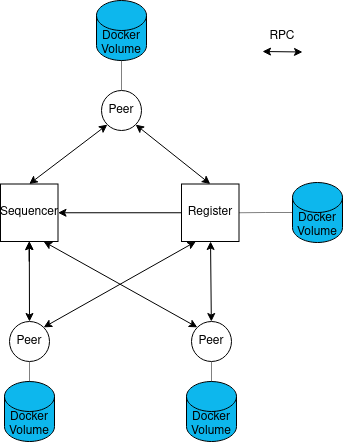
\includegraphics[width=0.25\textwidth]{architecture/architecture_1}}
\caption{Architettura algoritmo 1}
\end{figure} 

Si può notare dalla figura che ad ogni peer è stato montato un volume Docker, nel quale è presente il file utilizzato per simulare la consegna del messaggio a livello applicativo. 

Gli attori presenti nell'architettura sono:
\begin{itemize}
\item Il \textit{peer} rappresenta un partecipante al gruppo di multicast. Ovviamente, per poter partecipare alla comunicazione si ha la necessità di eseguire una registrazione ad esso.
\item Il \textit{register} rappresenta il nodo che permette di:
\begin{itemize}
\item Accettare le registrazione dei peer finché non si raggiunge il numero di partecipanti stabilito al gruppo multicast.
\item Inviare la lista dei peer partecipanti al gruppo ad ogni peer registrato.
\end{itemize}
\item Il \textit{sequencer} è il nodo che implementa l'algoritmo, assegnando un identificativo ad ogni pacchetto che permette di avere un ordinamento totale.
\end{itemize}

\subsubsection{Architettura per gli algoritmi 2 e 3}
L'architettura ideata per la realizzazione degli algoritmi 2 e 3 è la seguente.
\begin{figure}[ht!]
\centering
\frame{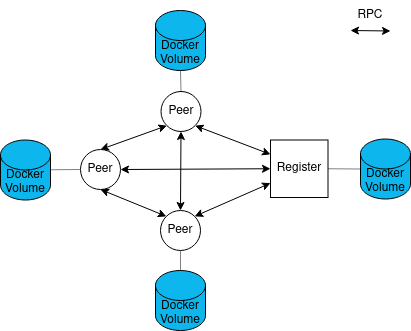
\includegraphics[width=0.3\textwidth]{architecture/architecture_2_3}}
\caption{Architettura algoritmi 2 e 3}
\end{figure}

Si può notare, come rispetto all'architettura precedente, non sia presente il \textit{sequencer} poiché gli algoritmi 2 e 3 sono algoritmi realizzati in modo distribuito.

\section{Implementazione}
In questa sezione saranno descritti i dettagli implementativi riguardante la realizzazione degli algoritmi.

\subsection{Orchestrazione dei container}
Per l'orchestrazione dei container è stato utilizzato \textit{Docker Compose}. In particolare, sono state fatte le seguenti scelte:
\begin{itemize}
\item È stata creata una rete virtuale per effettuare la comunicazione fra i diversi container up and running.
\item È stato creato un profilo \texttt{sequencer} che permette di adattare l'istanziazione dell'infrastruttura in base alla scelta dell'algoritmo. In particolare, se viene scelto l'algoritmo numero 1, il \texttt{sequencer} verrà istanziato, altrimenti esso non farà parte della struttura dell'applicazione.

Questo permette di avere una flessibilità dell'infrastruttura e di non sprecare risorse in caso in cui si utilizzino algoritmi diversi dall'1.
\item Sono state create delle variabili d'ambiente che permettono di avere dei parametri configurabili. In particolare, le variabili d'ambiente sono utilizzate per la scelta dell'algoritmo e per il numero di nodi partecipanti alla comunicazione multicast.
\end{itemize}

\subsection{Istanziazione dei container}
Per la gestione dell'istanziazione dei container è stato utilizzato \textit{Docker} e si è l'immagine di base selezionata è \texttt{golang:1.16-alpine} poiché ha una footprint minore rispetto, ad esempio, Ubuntu e conteniamo tutto ciò che è necessario per l'applicazione corrente.

Vengono sfruttate le variabili d'ambiente specificate nella sottosezione precedente per essere importate all'interno dell'applicazione \textit{Go}.

\subsection{Comunicazione fra i container}
I nodi, descritti nella sezione \ref{subsec:architetture}, comunicano fra loro attraverso il meccanismo di \textit{Remote Procedure Call}. Per l'implementazione di RPC non è stato utilizzato \texttt{gRPC}, ma è stato usato il package \texttt{"net/rpc"} poiché l'applicativo è totalmente scritto in \textit{Go} e quindi non si necessitava di una versatilità per quanto riguarda il linguaggio di programmazione.

In particolare, nelle prossime sottosezioni verrà descritto quali metodi sono esposti dal nodo e come è stata organizzata la loro struttura.

\subsection{Struttura di un peer}
Il peer è la figura più complessa che è stata gestita per la realizzazione di questo applicativo poiché, in base all'algoritmo da eseguire, esso ha dei compiti differenti.

È stata implementata una classe \texttt{Peer} che astrae e cattura le caratteristiche e funzioni di base di un semplice peer, in modo tale da specializzare questi aspetti in base allo scenario in cui essi si trovano.

Le caratteristiche di base di un peer individuate sono
\begin{itemize}
\item L'indice del processo\footnote{Gli algoritmi si basano anche sull'indice numerico del processo nel momento in cui si verificano situazioni particolari, quindi questa è stata pensata come una caratteristica chiave di un peer.};
\item L'indirizzo IP;
\item Il numero di porta;
\item L'username.
\end{itemize}

Le funzioni base di un peer sono:
\begin{itemize}
\item La registrazione all'interno del gruppo di multicast;
\item La ricezione della lista dei nodi registrati e la ricezione, da parte del frontend, del messaggio da inoltrare nella rete.
\end{itemize}

Per gli altri "tipi" di peer sono state realizzate altre classi (i.e. strutture in \textit{Go}) che vanno ad estendere la classe \texttt{Peer} appena descritte (i.e. la struttura \texttt{Peer} viene inglobata nelle nuove strutture). Ogni classe avrà i propri metodi, in modo tale che essi si adattino il miglior modo possibile all'algoritmo da realizzare.

Questo approccio ha permesso di avere un codice modulare che si adatta in base all'algoritmo richiesto poiché, nella fase di startup, è presente uno \texttt{switch} che ha il compito di individuare l'algoritmo da eseguire e di creare le corrette istanze dei peer.

\subsection{Dettagli implementativi per l'algoritmo 2}
Uno dei punti chiavi dell'implementazione dell'algoritmo 2 è sicuramente la realizzazione di una lista d'attesa dei messaggi di update ordinati in base al timestamp.

Per far fronte a questo aspetto, si è scelto di realizzare una lista collegata dove ogni nodo è rappresentato dal messaggio di update. Il punto chiave di questa implementazione è che l'inserimento in questa coda avviene in maniera ordinata, ovvero si scandisce la lista finché non si trova un nodo con timestamp maggiore del nodo candidato ad entrare e, dopo averlo trovato, viene inserito il nodo nella posizione corretta.

\section{Piattaforma software}
La piattaforma software utilizzata per la realizzazione dell'applicativo è la seguente:
\begin{itemize}
\item Il sistema operativo è Ubuntu 20.04.3 LTS;
\item Il linguaggio di programmazione utilizzato è \textit{Go};
\item Per l'istanziazione di ogni nodo è stato utilizzato \textit{Docker};
\item Per l'orchestrazione dei container è stato utilizzato \textit{Docker Compose}.
\end{itemize}

Per eseguire l'applicativo si ha bisogno solamente di aver istallato, all'interno della propria piattaforma software, \textit{Docker} perché permetterà di istanziare l'applicazione. 

\section{Testing dell'applicazione}
Per verificare il corretto comportamento degli algoritmi implementati sono stati ideati dei test. In particolare, per ogni algoritmo:
\begin{itemize}
\item Un test riguarda l'invio del messaggio di multicast da parte di un solo peer.
\item Un test riguarda l'invio del messaggio di multicast, anche in modo concorrente, da parte di più peer.
\end{itemize}

\subsection{Test per l'algoritmo 1}
\subsubsection{Un solo sender} In questa tipologia di test un peer invia sei messaggi, uno dopo l'altro in modo tale da rispettare l'assunzione \textit{FIFO} ordered.

Il risultato aspettato è che ogni peer consegni, nello stesso identico ordine, i messaggi ricevuti al livello applicativo.

\subsubsection{Più sender} In questa tipologia di test ogni peer, in modo concorrente, invia un messaggio al \textit{sequencer} e dopo aver inviato il primo messaggio, inoltra anche un secondo messaggio. 

Il risultato aspettato è che ogni peer consegni, nello stesso identico ordine, i messaggi ricevuti al livello applicativo.

\subsection{Test per l'algoritmo 2}
\subsubsection{Un solo sender} In questa tipologia di test un peer invia sei messaggi, uno dopo l'altro in modo tale da rispettare l'assunzione \textit{FIFO} ordered.

Il risultato aspettato è che nessun peer consegni messaggi a livello applicativo, in quanto non viene mai rispettata la condizione di consegna poiché è solamente un peer ad effettuare l'inoltro del messaggio in multicast.

\subsubsection{Più sender} In questa tipologia di test ogni peer, in modo concorrente, invia un messaggio al \textit{sequencer} e dopo aver inviato il primo messaggio, inoltra anche un secondo messaggio. 

Il risultato aspettato è che i primi $N$ messaggi consegnati al livello applicativo da ciascun peer siano i medesimi, dove $N$ è il numero minimo di messaggi consegnati dai peer.
\subsection{Test per l'algoritmo 3}
\subsubsection{Un solo sender} In questa tipologia di test un peer invia sei messaggi, uno dopo l'altro in modo tale da rispettare l'assunzione \textit{FIFO} ordered.

Il risultato aspettato è che ogni peer consegni, nello stesso identico ordine, i messaggi ricevuti al livello applicativo poiché, essendo un solo sender, non c'è relazione di causa-effetto fra i messaggi.

\subsubsection{Più sender} In questa tipologia di test si è seguito uno schema ben preciso per avere un test valido dal punto di vista della verifica. Lo schema è rappresentato nella seguente figura.

\begin{figure}[ht!]
\centering
\frame{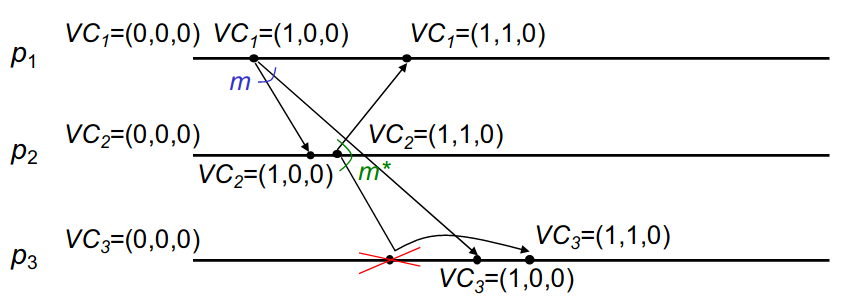
\includegraphics[width=0.45\textwidth]{architecture/test}}
\caption{Test per l'algoritmo 3}
\end{figure}

In particolare, lo scenario è il seguente:
\begin{itemize}
\item Il peer $p_1$ invia un messaggio con timestamp $(1, 0, 0)$ in multicast. Questo messaggio viene ricevuto dal peer $p_2$, ma a causa di un ritardo non viene ricevuto subito dal peer $p_3$.
\item Il peer $p_2$, a causa del messaggio ricevuto, inoltra un messaggio in multicast con timestamp $(1, 1, 0)$. Questo messaggio viene ricevuto da entrambi i peer senza ritardi. 
\item Il peer $p_3$, al momento della ricezione del messaggio inviato da $p_2$, deve posticipare la consegna del messaggio con timestamp $(1, 1, 0)$. Una volta ricevuto e consegnato il messaggio con timestamp $(1, 0, 0)$, può procedere con la consegna del messaggio inviato da $p_2$.
\end{itemize}

Il risultato aspettato è che tutti i peer consegnino i messaggi rispettando la relazione di causa-effetto. Quindi, in questo caso significa che ogni peer consegni, nello stesso ordine, i due messaggi al livello applicativo.



\end{document}
\endinput
%%
%% End of file `sample-acmtog.tex'.
